%% VerifiQuant — dual-target draft (sigconf)
%% Page budgets: FinNLP = 8 pages of BODY (refs excluded, appendix unlimited);
%%               ICAIF  = 8 pages ALL-INCLUSIVE (refs counted, no appendix, desk reject if over).
%% Strategy: this file carries the FULL (FinNLP-sized) content. Blocks marked
%%   %% [ICAIF-CUT] ... %% [/ICAIF-CUT]
%% are the pre-agreed trim candidates for the ICAIF 8-page all-in version.
%% Numbers that may still change live in numbers.tex.
\documentclass[sigconf,review,anonymous]{acmart}
\usepackage{booktabs}
\usepackage{pgfplots}
\pgfplotsset{compat=1.18}
% numbers.tex — single source of truth for result numbers that may still change.
% ⚠ VQ 250Q values below are from run1 (pre scalar-fix cards). When the repaired-card
%   rerun lands, update ONLY this file. Provenance: docs/2026-07-12_experiment_record_master.md

% ── VerifiQuant, 250Q, K=3 (Flash) ──
\newcommand{\vqCorrectAll}{231}
\newcommand{\vqAccAll}{92.4\%}
\newcommand{\vqSWAll}{10}
\newcommand{\vqAbstainAll}{9}
\newcommand{\vqCovAll}{96.4\%}
\newcommand{\vqSelAccAll}{95.9\%}
\newcommand{\vqSWRAll}{4.0\%}
\newcommand{\vqCorrectMed}{172}
\newcommand{\vqSWMed}{3}
\newcommand{\vqAbstainMed}{5}
\newcommand{\vqSWRMed}{1.7\%}
\newcommand{\vqSelAccMed}{98.3\%}
\newcommand{\vqCorrectHard}{59}
\newcommand{\vqSWHard}{7}
\newcommand{\vqAbstainHard}{4}
\newcommand{\vqSWRHard}{10.0\%}
\newcommand{\vqSelAccHard}{89.4\%}
% SWR improvement ratios vs CoT single-shot (13.9 / 28.6 / 18.0)
\newcommand{\vqSWRatioMed}{8.2$\times$}
\newcommand{\vqSWRatioHard}{2.9$\times$}
\newcommand{\vqSWRatioAll}{4.5$\times$}
% residual-failure attribution counts (class A already repaired in canonical run)
\newcommand{\swResidual}{10}
\newcommand{\swClassA}{3}
\newcommand{\swClassB}{2}
\newcommand{\swClassC}{2}
\newcommand{\swClassD}{3}

% ── CoT single-shot, 250Q (honest ternary accounting) ──
\newcommand{\cotCorrectAll}{194}
\newcommand{\cotAccAll}{77.6\%}
\newcommand{\cotSWAll}{45}
\newcommand{\cotAbstainAll}{11}
\newcommand{\cotSWRAll}{18.0\%}
\newcommand{\cotSelAccAll}{81.2\%}
\newcommand{\cotSWRMed}{13.9\%}
\newcommand{\cotSWRHard}{28.6\%}
\newcommand{\cotCorrectMed}{148}\newcommand{\cotSWMed}{25}\newcommand{\cotAbstainMed}{7}
\newcommand{\cotCorrectHard}{46}\newcommand{\cotSWHard}{20}\newcommand{\cotAbstainHard}{4}

% ── CoT + GT-blind oracle (K=3), 250Q ──
\newcommand{\cotoCorrectAll}{205}
\newcommand{\cotoAccAll}{82.0\%}
\newcommand{\cotoSWAll}{37}
\newcommand{\cotoAbstainAll}{8}
\newcommand{\cotoSWRAll}{14.8\%}
\newcommand{\cotoSelAccAll}{84.7\%}
\newcommand{\cotoSWRMed}{11.1\%}
\newcommand{\cotoSWRHard}{24.3\%}
\newcommand{\cotoCorrectMed}{157}\newcommand{\cotoSWMed}{20}\newcommand{\cotoAbstainMed}{3}
\newcommand{\cotoCorrectHard}{48}\newcommand{\cotoSWHard}{17}\newcommand{\cotoAbstainHard}{5}


\settopmatter{printacmref=false}
\renewcommand\footnotetextcopyrightpermission[1]{}
\pagestyle{plain}

\acmConference[ICAIF '26]{7th ACM International Conference on AI in Finance}{November 2026}{TBD}

\begin{document}

\title{VerifiQuant: Governance-by-Execution for Financial LLM Workflows}

\author{Anonymous Author(s)}
\affiliation{\institution{Anonymous Institution}\country{}}

\begin{abstract}
Large language models are increasingly embedded in financial workflows, yet they are governed---if at all---by prompts and post-hoc review.
We argue that the central deployment risk is not accuracy but \emph{governability}: a production financial AI system must declare its scope boundaries, refuse structurally when it cannot verify its own reasoning, expose replayable decision traces, and mathematically verify any repair it applies.
We present \textbf{VerifiQuant}, a framework that compiles these governance controls into the reasoning pipeline itself.
Each financial formula family is represented as a \emph{Financial Inference Contract} (FIC)---retrieval metadata, deterministic executable code, invariants, and declared semantic ambiguities---and every query passes through a six-layer diagnostic funnel in which each layer (M, N, F, E, I, C) is a legitimate, auditable exit.
Semantic repairs are restricted to \emph{verifiable atomic transforms} whose numerical effect is cross-checked against a declared algebraic identity before acceptance.
On 250 FinanceReasoning questions spanning medium and hard tiers, VerifiQuant reaches \vqAccAll{} accuracy with a silent-wrong rate of \vqSWRAll{}, dominating chain-of-thought baselines on \emph{both} axes simultaneously: the strongest CoT+oracle configuration reaches \cotoAccAll{} accuracy with \cotoSWRAll{} SWR, and the gap widens with difficulty (\vqSWRatioMed{} lower SWR on the medium tier, \vqSWRatioHard{} on hard).
Every residual VerifiQuant failure is attributed to one of three named frontier gaps---and mechanizing one of them (declared-hint recall) already cuts overall SWR to 1.2\% and the medium tier to 0\%, at an explicit 1.6-point coverage cost.
On contract-grounded adversarial traps the funnel cuts silent-wrong rates from 90\% to 20\% (boundary violations) and 100\% to 10\% (ambiguity).
Critically, governance does not transfer through prompts: injecting the complete diagnostic taxonomy into oracle prompts \emph{degrades} accuracy under blind review, and prompted refusal misfires on the wrong questions.
Governance must be executed by architecture, not described in context.
\end{abstract}

\begin{CCSXML}
<ccs2012>
<concept><concept_id>10010405.10003550</concept_id><concept_desc>Applied computing~Economics</concept_desc><concept_significance>500</concept_significance></concept>
<concept><concept_id>10010147.10010178</concept_id><concept_desc>Computing methodologies~Artificial intelligence</concept_desc><concept_significance>500</concept_significance></concept>
</ccs2012>
\end{CCSXML}
\ccsdesc[500]{Applied computing~Economics}
\ccsdesc[500]{Computing methodologies~Artificial intelligence}
\keywords{financial reasoning, LLM governance, selective prediction, neuro-symbolic systems, auditability}

\maketitle

\section{Introduction}
Financial institutions are deploying large language models (LLMs) in workflows that end in numbers: valuation memos, portfolio analytics, client-facing calculators, regulatory reports.
Benchmark accuracy on financial question answering has climbed steadily, and it is tempting to treat the remaining gap as an accuracy problem---one more model generation away from solved.
We argue this framing misses what actually blocks deployment.
A financial LLM workflow fails in production not primarily because it computes the wrong number, but because \emph{nobody can govern how it computes any number}.
Three failure modes, all invisible to headline accuracy, illustrate the gap.

\emph{Silent wrongs.}
The model outputs a confident, well-formatted, wrong number, with no signal distinguishing it from a correct one.
In our experiments a chain-of-thought (CoT) baseline produces confident unflagged wrong answers on \cotSWRAll{} of 250 financial questions---\cotSWRHard{} on the hard tier---and on adversarially perturbed inputs, up to 100\% for some perturbation classes (\S\ref{sec:trap}).

\emph{Audit gaps.}
When a loss occurs, the institution must reconstruct \emph{which} formula was applied, \emph{which} inputs were bound, and \emph{why} the system did not stop.
CoT traces cannot serve this role: they are sampled, non-reproducible, and---as the faithfulness literature shows---not causally connected to the computation that produced the answer \cite{turpin2023language,lanham2023measuring}.
Notably, this disconnect \emph{worsens} with model capability, so waiting for stronger models does not close the audit gap.

\emph{Boundary failures.}
Asked a question outside its competence---an exotic derivative it has no procedure for---the system answers anyway, often by silently substituting a different question it \emph{can} answer (\S\ref{sec:cases} shows a baseline pricing a ``Heston stochastic volatility'' request by computing an unrelated manufacturing ratio).

Regulatory frameworks for high-risk AI---model-risk guidance \cite{fed2011sr117}, the EU AI Act's logging provisions \cite{euaiact2024}, FINRA's supervisory-control expectations \cite{finra2020ai}---converge on a common demand: systems must declare their boundaries, log reproducibly, expose checkpoints for human intervention, and constrain internal modification (\S\ref{sec:governance}).
Today these demands are met, when at all, by \emph{prompt instructions} and \emph{post-hoc review}: governance described in natural language and hoped for at runtime.

\textbf{Our position is that governance controls must be executed, not described.}
VerifiQuant is built around three mechanisms.
(1)~\emph{Financial Inference Contracts (FICs)}: each formula family is compiled offline into a machine-readable contract---retrieval metadata, typed inputs, deterministic executable Python, numerical invariants and scale checks, and \emph{declared semantic ambiguities} (period timing, percent vs.\ decimal conventions, unit bases). The LLM never performs arithmetic; it selects contracts, binds fields, and flags ambiguities, all within contract-declared bounds.
(2)~\emph{A six-layer diagnostic funnel} (M/N/F/E/I/C): every query passes gates for intent (M), scope (N), schema completeness (F), boundary validity (E), semantic ambiguity (I---split into blocking I\textsubscript{HARD} and warning I\textsubscript{SOFT}), and deterministic computation (C). Each gate is a legitimate, structured exit carrying machine-readable diagnostics rather than prose apologies.
(3)~\emph{Verifiable atomic transforms}: when clarification changes the required computation, repairs are restricted to bounded transforms accepted only if their numerical effect matches a declared algebraic identity under cross-verification.

\textbf{Contributions.}
\begin{itemize}
\item We reframe financial LLM reliability as a governance problem and derive six executable controls from regulatory requirements (Table~\ref{tab:spine}), mapping each to an architectural mechanism and an experimental test.
\item We present the FIC + diagnostic-funnel architecture with verifiable atomic transforms (\S\ref{sec:method}), making refusal, clarification, and repair first-class auditable outcomes.
\item On 250 FinanceReasoning \cite{tang2025financereasoning} questions (180 medium + 70 hard), VerifiQuant dominates CoT baselines on accuracy \emph{and} silent-wrong rate simultaneously (\vqAccAll{} / \vqSWRAll{} vs.\ \cotoAccAll{} / \cotoSWRAll{} for the strongest baseline), with the SWR gap widening under difficulty shift (\S\ref{sec:results}); every residual failure is attributed to a named frontier gap (\S\ref{sec:attribution}).
\item We show governance does not transfer through prompts: describing the full diagnostic taxonomy to an oracle \emph{degrades} it under blind review, and prompted refusal is non-selective (\S\ref{sec:promptsnotcontrols}). We further localize the I-gate's binding constraint to \emph{declared-hint recall} and show a deterministic trigger pre-pass recovers it (\S\ref{sec:recall}).
\end{itemize}

\section{The Governance Problem}\label{sec:governance}

\subsection{What deployment actually requires}
Model-risk guidance (SR~11-7) requires that a model \emph{identify its own failure regimes} and enforce output boundaries rather than extrapolate \cite{fed2011sr117}.
The EU AI Act (Art.~12--13) requires event logging sufficient to \emph{trace any output back to its inputs}, reproducibly \cite{euaiact2024}.
FINRA supervisory guidance requires \emph{explicit human checkpoints} where the system cannot autonomously resolve ambiguity, and that internal modifications be bounded and reviewable \cite{finra2020ai}.
Table~\ref{tab:spine} restates these demands as six concrete controls, each paired with the mechanism that executes it and the experiment that tests it; \S\ref{sec:method} walks the mechanism column, \S\ref{sec:results}--\ref{sec:analysis} the evidence column.

\begin{table}[t]
\caption{Governance controls $\rightarrow$ executing mechanism $\rightarrow$ evidence.}
\label{tab:spine}
\small
\begin{tabular}{@{}p{0.16\linewidth}p{0.30\linewidth}p{0.40\linewidth}@{}}
\toprule
Control & Mechanism (\S\ref{sec:method}) & Evidence \\
\midrule
C1 boundary declaration & M/N structured refusal & trap-N/M; MAS baseline lacks it $\rightarrow$ 14\% SWR \\
C2 input validation & deterministic E-checks & trap-E: SWR 90\%$\rightarrow$20\% \\
C3 ambiguity disclosure & I\textsubscript{HARD} block / I\textsubscript{SOFT} warning & trap-I: SWR 100\%$\rightarrow$10\% \\
C4 verified repair & atomic transforms (AST + numeric cross-verify) & worked example \S\ref{sec:transforms} \\
C5 replayable trace & DiagnosticReport + deterministic execution & 4 reruns: accuracy/SWR variance $=0$ \\
C6 abstention as control & selective-prediction exits at every gate & residual-failure attribution \S\ref{sec:attribution} \\
\bottomrule
\end{tabular}
\end{table}

\subsection{Why existing approaches do not provide these controls}
\emph{Execution-based reasoning} (PAL \cite{gao2023pal}, Program-of-Thoughts \cite{chen2023pot}) delegates arithmetic to an interpreter, addressing C-class errors; but a syntactically perfect program can encode the wrong financial semantics---an end-of-period annuity where the question implies beginning-of-period---and the interpreter neither detects this nor produces structured attribution.
\emph{Neuro-symbolic translation} (Logic-LM \cite{pan2023logiclm}, LINC \cite{olausson2023linc}, SATLM \cite{ye2023satlm}) obtains formal guarantees by translating natural language into solver input, but the translation step is the dominant error source, and recent analysis argues specification synthesis is undecidable in general \cite{zhou2026formaljudge}.
VerifiQuant moves the formalization burden \emph{offline}: contracts are built and validated at build time, so runtime only selects and binds within a pre-verified space.
\emph{Multi-agent and self-reflection systems} rely on natural-language consensus between agents; failures propagate silently across agent boundaries \cite{cemri2025mas}.
We reimplement a nine-node financial multi-agent system \cite{kundu2025multiagent} and find that even with oracle support it never triggers its own \texttt{ask\_human} node, delivering 14\% SWR (\S\ref{sec:fiftyq})---an architecture with a human-checkpoint \emph{node} but no executed \emph{control} that routes to it.
\emph{Prompted refusal} is the cheapest candidate control; \S\ref{sec:promptsnotcontrols} shows it is non-selective.

\section{Method}\label{sec:method}

\subsection{Financial Inference Contracts}
An FIC packages one formula family as three artifacts keyed by \texttt{fic\_id}.
The \emph{retrieval card} carries selection hints, applicability and non-applicability conditions, scope boundaries, and keywords, used by BM25 plus an LLM selector to decide whether the contract applies.
The \emph{core card} carries typed inputs, deterministic \texttt{compute} code in plain Python, numerical invariants and scale checks (E-checks), and \texttt{semantic\_hints} declaring known ambiguities---each with resolution options, a default, and a hard/soft level.
The \emph{repair card} maps each diagnostic outcome to one of eight structured actions (request missing fields, present clarification options, declare scope boundary, \ldots), each declaring its legal next-step transitions.
The LLM's role is \emph{mapping into contracts}---selecting, binding, flagging---never computing.
Contracts are themselves governed at build time: E-check expressions are lint-gated against the exact evaluation namespace used at runtime, every card passes execution smoke tests, and a pre-declared output-type policy is enforced by audit (\S\ref{sec:attribution} shows this audit catching real defects).

\subsection{The M/N/F/E/I/C diagnostic funnel}
Given a question and context, gates fire in order:
\textbf{M} (intent): does the question map to exactly one contract family? Exit: structured disambiguation request.
\textbf{N} (scope): is any contract applicable? Exit: scope-boundary refusal.
\textbf{F} (schema): are all required inputs present? Exit: slot-filling request with \texttt{requested\_fields}.
\textbf{E} (boundary): do bound inputs satisfy invariants and scale checks? Exit: deterministic alert naming the violated check.
\textbf{I} (ambiguity): does an unresolved declared ambiguity change the computation (I\textsubscript{HARD}: block and clarify) or only its interpretation (I\textsubscript{SOFT}: proceed with explicit warning)?
\textbf{C}: deterministic execution with audit log.
Every case yields a $\mathrm{DiagnosticReport}=(\textit{exit\_layer},\textit{fic\_id},\textit{binding},\textit{invariant\_trace},\textit{action})$: replayable, layer-attributable, machine-readable.
Abstention is not a fallback; it is the designed output of five of the seven gates (C6).
Figure~\ref{fig:pipeline} annotates each gate with the control it executes.

\begin{figure*}[t]
\centering
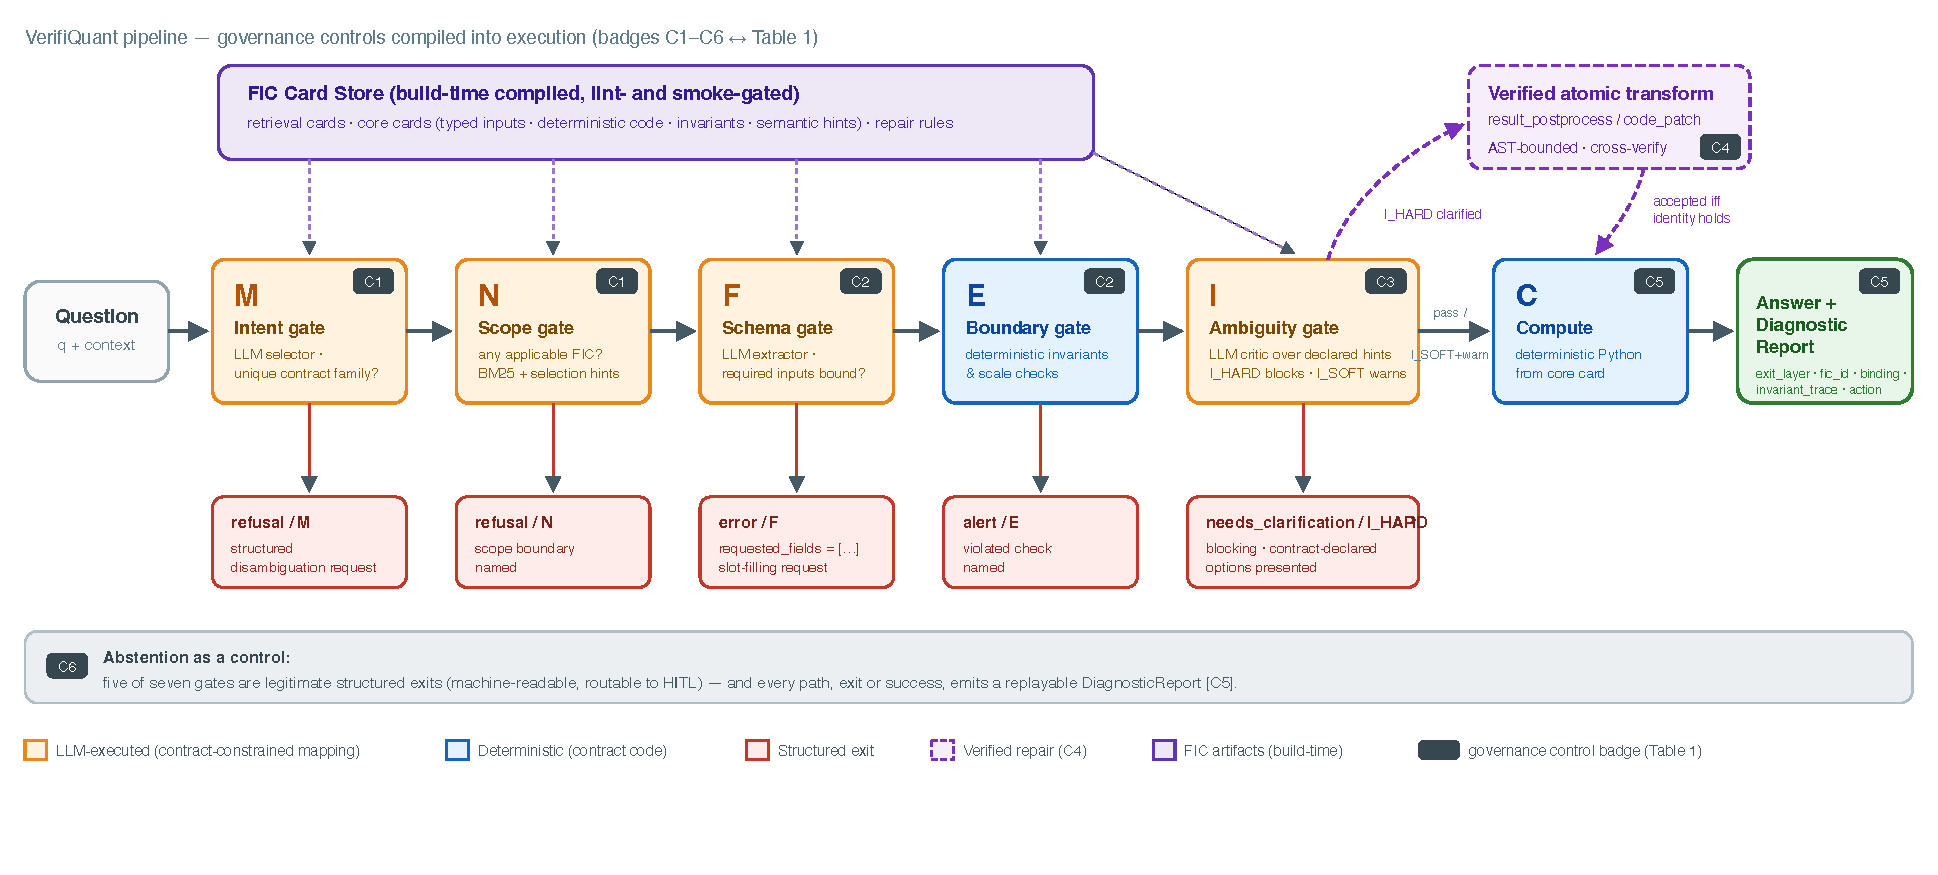
\includegraphics[width=\textwidth]{figures/fig1_pipeline.pdf}
\caption{The VerifiQuant pipeline. LLM components (orange) only map into contracts; all financially consequential computation is deterministic (blue). Five of seven gates are structured exits (red); repairs go through verified atomic transforms (purple). Badges C1--C6 reference Table~\ref{tab:spine}.}
\label{fig:pipeline}
\end{figure*}

\subsection{Oracle-in-the-loop evaluation protocol}\label{sec:oitl}
To measure \emph{recoverability}---how far the framework gets when intent is clear but the answer is unknown---a constrained oracle agent simulates an ideal clarifying user.
Per turn the oracle reads the current DiagnosticReport and the question's ground-truth \emph{computation code} (the intent specification) but never the numeric answer; it may only rewrite question/context, never inject values.
Iteration is capped at $K{=}3$.
The same GT-blind discipline applies to all CoT+oracle baselines: the oracle reviews every turn (blind review), receives no correctness signal, and never sees the numeric ground truth---otherwise ``intervene only when wrong'' itself leaks the label.
Across all oracle configurations $\mathrm{broken\_count}=0$: blind review never corrupted a correct answer.

\subsection{Verifiable atomic transforms}\label{sec:transforms}
When an I\textsubscript{HARD} clarification changes the required computation, free-form code regeneration would reopen the door the funnel just closed.
VerifiQuant permits exactly two repair forms.
\emph{result\_postprocess}: a pure-arithmetic expression over the original result and bound inputs (e.g., $r \times (1+i)$), bounded by an AST node-count limit, a safe-name whitelist, and a numerical invariant check.
\emph{code\_patch}: a single-site textual replacement in contract code (e.g., \texttt{start=1} $\rightarrow$ \texttt{start=0}), accepted only if the pattern occurs exactly once, the shallow AST diff is within a declared blast radius, no new imports or dangerous calls appear, and---decisively---\emph{cross-verification}: the patched code's output must equal the declared algebraic identity applied to the original output on multiple sampled inputs.
\emph{Worked example (annuity timing).} A contract computes an end-of-period annuity (579.98). The user clarifies payments occur at period start. The system applies the pre-declared post-process \emph{and} the code patch, reruns, and compares: both yield 577.10, so the repair is accepted and logged with its invariant. A code change is admissible only when its numerical effect is provable without trusting the LLM that proposed it (C4).

%% [ICAIF-CUT: design-rationale subsection]
\subsection{Design rationale: alternatives we rejected}\label{sec:rationale}
Three designs we prototyped or evaluated en route shaped the final architecture; each fails for a reason that clarifies what the controls actually require.
\emph{(a) One-shot symbolic compilation.}
Compiling all financial logic up front into a solver-executable policy space (SMT-lib policies over accounting and regulatory rules \cite{akinfaderin2025verafi}, or deterministic rule graphs) yields near-perfect logical consistency \emph{after} translation---but a single error in that one-shot translation poisons every downstream execution, and the rigid policy space resists the heterogeneous phrasing of real questions.
FICs amortize formalization per formula family instead: each contract is validated independently at build time, a bad card damages only its own family, and selection keeps a natural-language interface.
\emph{(b) Symbolic-proof transforms.}
Our first transform design attached a computer-algebra proof to each repair (e.g., $\mathrm{PV}_{\mathrm{due}}=\mathrm{PV}_{\mathrm{ord}}\times(1+r)$, checked with a CAS).
We dropped the solver: the proof catalog needs manual maintenance, and the natural-language-to-symbolic translation it depends on is itself the dominant failure mode identified in \S\ref{sec:governance}.
Numerical cross-verification of the declared identity on sampled inputs yields the same accept/reject decision with no symbolic dependency.
\emph{(c) Probabilistic belief fusion.}
Reasoning-in-action systems that anchor claims to calibrated confidence scores answer ``how sure are we?''---but a calibrated 0.85 cannot answer \emph{which check failed}, and finance's near-zero error tolerance demands exact attribution, not belief updates.
The common thread: every rejected design either centralizes a fragile translation step or reports uncertainty without attribution; the funnel decentralizes the former and structurally provides the latter.
%% [/ICAIF-CUT]

\section{Experimental Protocol}\label{sec:protocol}

\subsection{Datasets}
\textbf{Clean set (main).} 250 questions from FinanceReasoning \cite{tang2025financereasoning}: 180 medium (difficulty 2.48--4.14) and 70 hard (4.16--7.19), stratified by difficulty quartile at seed 42; question IDs are committed.
The hard tier probes governance behavior under difficulty shift.
A canonical 50-question medium subset supports deep protocol validation (full oracle grid, ablations, variance; \S\ref{sec:fiftyq}).
FIC cards are auto-generated per question family and validated by build-time gates (execution smoke: 0 failures; E-check lint: 4 statement-form expressions on 2 cards repaired pre-run; cross-artifact relation check: clean); all repairs are logged and none consults gold answers.
\emph{Contamination control.}
An early pipeline built cards from each question's reference \emph{solution}---effectively compiling the test set into the knowledge base and mass-producing near-duplicate cards.
The final protocol generates cards only from the benchmark's independent reference-function corpus (article-level implementations published separately from the questions), never receives gold answers or per-question solution code, and deduplicates formula kernels by AST hashing.

\textbf{Trap set (contract-grounded).} Trap labels guessed from question text are themselves unreliable, so each trap is derived from a clean question plus its FIC by a deterministic operator---the label \emph{is} the operator.
\textbf{F} removes a required input; \textbf{E} injects a boundary-violating value anchored to a declared E-check predicate; \textbf{I} deletes the disambiguating phrase that re-opens a declared semantic hint (hard/soft per the contract); \textbf{N} swaps in an out-of-scope ask while keeping the original context; \textbf{M} replaces the question with under-specified intent.
50 traps (10 per operator), zero \texttt{needs\_review}, manually spot-checked.
%% [ICAIF-CUT: operator examples]
Concretely: an E-trap sets total revenue to $-\$1.2$M (financially absurd, syntactically legal); an I-trap deletes ``expressed as a percentage'', re-opening a declared decimal/percent hint; an N-trap asks for Heston stochastic-volatility pricing over an untouched manufacturing context.
%% [/ICAIF-CUT]
\emph{Honest scoping:} N is defined relative to the contract library (a principled OOD check for VerifiQuant, an incidental mismatch cue for CoT), and the Tier-1 M operator retains metric-bearing context, limiting what M results can claim (\S\ref{sec:trap}).

\subsection{Baselines and metrics}
On 250Q: CoT single-shot (Gemini 2.5 Flash), CoT + GT-blind oracle ($K{=}3$, blind review), VerifiQuant ($K{=}3$, Flash).
On the canonical 50Q: additionally CoT single-shot/oracle with Gemini 2.5 Pro, plain and funnel-guided oracle prompts, a J.P.\ Morgan multi-agent reimplementation \cite{kundu2025multiagent}, and VerifiQuant Pro.
Following selective prediction \cite{elyaniv2010foundations,geifman2017selective}, every case is \emph{Correct}, \emph{Silent Wrong} (confident unflagged wrong number), or \emph{Abstention}; informal no-answers (a model declining in prose, without diagnostics) are counted as abstention, not silent wrong, for \emph{all} systems.
We report coverage, selective accuracy $=$ Correct/(Correct$+$SW), and \textbf{SWR} $=$ SW$/N$---the key deployment-risk metric.
On traps, where no legitimate numeric answer exists, correct behavior is interception; we report trap SWR and the structured-catch rate.

\section{Results}\label{sec:results}

\subsection{Main results: 250 questions, two difficulty tiers}
Table~\ref{tab:main} is the headline result.
VerifiQuant dominates both CoT configurations on \emph{both} axes simultaneously: accuracy \vqAccAll{} vs.\ \cotoAccAll{} (strongest baseline) and SWR \vqSWRAll{} vs.\ \cotoSWRAll{}.
The oracle helps CoT (77.6\%$\rightarrow$82.0\%) but does not change its failure mode: coverage stays effectively forced, and roughly one answer in seven is a confident unflagged wrong number.

\begin{table*}[t]
\caption{Main results on 250 FinanceReasoning questions (180 medium / 70 hard), Gemini 2.5 Flash. SW $=$ silent wrong; Abst $=$ abstention (VerifiQuant: structured, diagnostic-bearing; CoT: informal no-answers, counted charitably as abstention). All oracles are GT-blind (\S\ref{sec:oitl}).}
\label{tab:main}
\small
\begin{tabular}{@{}llrrrrrr@{}}
\toprule
System & Tier & $N$ & Correct & SW & Abst & Sel.\ Acc & SWR \\
\midrule
CoT single-shot & medium & 180 & \cotCorrectMed{} & \cotSWMed{} & \cotAbstainMed{} & 85.5\% & \cotSWRMed{} \\
 & hard & 70 & \cotCorrectHard{} & \cotSWHard{} & \cotAbstainHard{} & 69.7\% & \cotSWRHard{} \\
 & all & 250 & \cotCorrectAll{} & \cotSWAll{} & \cotAbstainAll{} & \cotSelAccAll{} & \cotSWRAll{} \\
\midrule
CoT + blind oracle ($K{=}3$) & medium & 180 & \cotoCorrectMed{} & \cotoSWMed{} & \cotoAbstainMed{} & 88.7\% & \cotoSWRMed{} \\
 & hard & 70 & \cotoCorrectHard{} & \cotoSWHard{} & \cotoAbstainHard{} & 73.8\% & \cotoSWRHard{} \\
 & all & 250 & \cotoCorrectAll{} & \cotoSWAll{} & \cotoAbstainAll{} & \cotoSelAccAll{} & \cotoSWRAll{} \\
\midrule
\textbf{VerifiQuant ($K{=}3$)} & medium & 180 & \vqCorrectMed{} & \vqSWMed{} & \vqAbstainMed{} & \vqSelAccMed{} & \textbf{\vqSWRMed{}} \\
 & hard & 70 & \vqCorrectHard{} & \vqSWHard{} & \vqAbstainHard{} & \vqSelAccHard{} & \textbf{\vqSWRHard{}} \\
 & all & 250 & \vqCorrectAll{} & \vqSWAll{} & \vqAbstainAll{} & \vqSelAccAll{} & \textbf{\vqSWRAll{}} \\
\midrule
\quad + hint triggers (\S\ref{sec:recall}) & medium & 180 & \vqtCorrectMed{} & \vqtSWMed{} & \vqtAbstainMed{} & \vqtSelAccMed{} & \textbf{\vqtSWRMed{}} \\
 & hard & 70 & \vqtCorrectHard{} & \vqtSWHard{} & \vqtAbstainHard{} & \vqtSelAccHard{} & \vqtSWRHard{} \\
 & all & 250 & \vqtCorrectAll{} & \vqtSWAll{} & \vqtAbstainAll{} & \vqtSelAccAll{} & \textbf{\vqtSWRAll{}} \\
\bottomrule
\end{tabular}
\end{table*}

\textbf{Difficulty shift is a governance stress test.}
Moving from medium to hard \emph{doubles} CoT's silent-wrong rate (\cotSWRMed{}$\rightarrow$\cotSWRHard{} single-shot; \cotoSWRMed{}$\rightarrow$\cotoSWRHard{} with oracle): harder questions convert directly into more confident wrong numbers, with no signal.
VerifiQuant's SWR stays in a narrow band (\vqSWRMed{}$\rightarrow$\vqSWRHard{}): the contract gates and abstention absorb most of the shift, so the advantage over CoT \emph{widens} with difficulty---\vqSWRatioMed{} on medium, \vqSWRatioHard{} on hard (Figure~\ref{fig:tiers})---and, unlike CoT, every residual failure is attributable (\S\ref{sec:attribution}).

\begin{figure}[t]
\centering
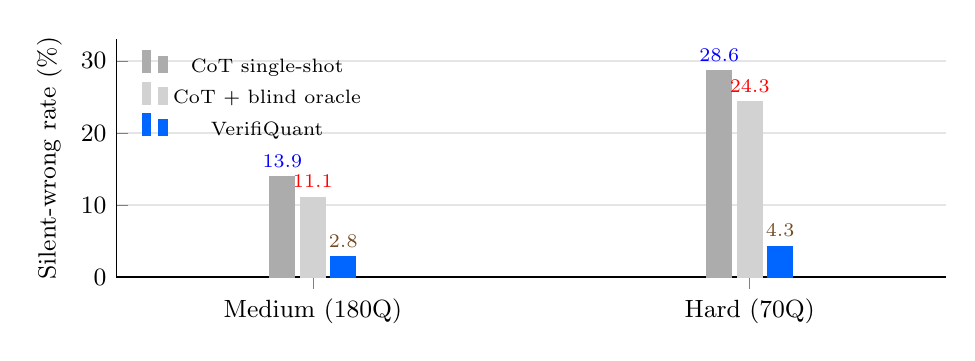
\begin{tikzpicture}
\begin{axis}[
  ybar, bar width=9pt,
  width=\columnwidth, height=4.6cm,
  ymin=0, ymax=33,
  ylabel={Silent-wrong rate (\%)},
  ylabel near ticks,
  symbolic x coords={Medium (180Q), Hard (70Q)},
  xtick=data,
  enlarge x limits=0.45,
  legend style={at={(0.02,0.98)}, anchor=north west, font=\scriptsize, draw=none, fill=none},
  nodes near coords, nodes near coords style={font=\scriptsize},
  tick label style={font=\small},
  label style={font=\small},
  axis lines*=left, ymajorgrids, grid style={gray!20},
]
\addplot+[ybar, fill=gray!65, draw=gray!65] coordinates {(Medium (180Q),13.9) (Hard (70Q),28.6)};
\addplot+[ybar, fill=gray!35, draw=gray!35] coordinates {(Medium (180Q),11.1) (Hard (70Q),24.3)};
\addplot+[ybar, fill=blue!60!cyan, draw=blue!60!cyan] coordinates {(Medium (180Q),2.8) (Hard (70Q),4.3)};
\legend{CoT single-shot, CoT + blind oracle, VerifiQuant}
\end{axis}
\end{tikzpicture}
\caption{Difficulty shift as a governance stress test. Hard-tier questions roughly double CoT's silent-wrong rate under both configurations; VerifiQuant's stays in a narrow band, so its advantage widens from \vqSWRatioMed{} to \vqSWRatioHard{}.}
\label{fig:tiers}
\end{figure}

\subsection{Residual-failure attribution and the audit loop}\label{sec:attribution}
Fifty-question pilots of this framework achieved SWR $=0\%$; at 250 questions with a hard tier, silent wrongs appear.
We attribute \emph{every} one.
The \swResidual{} silent wrongs of the initial 250Q run decompose into four classes.
(The canonical numbers in Table~\ref{tab:main} are from the post-audit rerun described under class~A below; we narrate the initial run first because the audit is part of the result.)
\textbf{(A) Output-policy violations (\swClassA{}, all hard).} Three time-series indicator cards (NVI, VPT, VWAP) compute the correct value series but return the whole list, violating the pre-declared scalar-output policy; the runtime surfaced the first element while the series-final value matches gold.
Because the policy predates the run, this is detectable \emph{without gold answers}: a type audit of all 250 cards (dynamic replay of every card--input pair used in the run, plus a static AST scan) found exactly these plus one dict-returning card, auto-repaired all four with logged diffs, flagged two deliberately-array cards for review, and cleared three false positives.
This audit-repair cycle is governance-by-execution applied to the system itself: the failure was localized to specific contract lines, repaired under a pre-declared policy, and both runs are preserved.
\textbf{(B) Selection mismatch (\swClassB{}).} Two ``total interest'' questions were routed to an internally-correct ``lifetime cost'' card (outputs differ by exactly the principal): an M-layer frontier failure, not a computation error.
\textbf{(C) Binding slips (\swClassC{}).} The extractor bound a wrong-but-legal value (e.g., the annualization base 360 where the 90-day tenor was required): the input-provenance gap of \S\ref{sec:limitations}.
\textbf{(D) Declared-but-unrecalled ambiguities (\swClassD{}).} Most instructive: in all three cases the selected card \emph{already declares} the exact ambiguity as a semantic hint (per-share vs.\ total premium; percent vs.\ decimal output; sign convention of working-capital changes), yet the LLM critic failed to trigger it---declaration coverage 3/3, recall 0/3 (\S\ref{sec:recall}).

After the class-A repair, the canonical rerun (Table~\ref{tab:main}) has \swResidualCanon{} silent wrongs---all from the \emph{same three frontier families} (\swCanonB{} selection, \swCanonC{} binding, \swCanonD{} convention), with zero unattributed: five persist from the initial run and three are sampling-variant instances of the same families (two of the initial convention cases resolve correctly under resampling, confirming that class~D behaves as an unflagged coin flip---precisely what I\textsubscript{SOFT} disclosure exists to prevent).
On the canonical 50-question subset the audited cards score 50/0/0.

\subsection{Protocol validation on the canonical 50Q subset}\label{sec:fiftyq}
The 50Q medium subset carries the full baseline grid (Table~\ref{tab:fifty}).
Three findings transfer.
(1)~\emph{Oracle strength does not eliminate silent wrongs}: the strongest leak-free configuration (plain oracle, Pro) reaches 98\% accuracy yet keeps SWR $\geq2\%$; its surviving error is architectural---LLM arithmetic on $2.4^{1/5}$ oscillates across turns (19.11--19.16), which no clarification can fix and deterministic execution computes exactly.
(2)~\emph{A multi-agent system with a human-escalation node never uses it}: the MAS baseline answered all 50 questions without once triggering \texttt{ask\_human} (SWR 14\%)---possessing a checkpoint is not executing one.
%% [ICAIF-CUT: MAS failure color]
Its failure modes, observed during reimplementation, are instructive: after several rounds of inter-agent chatter the base agent starts ignoring provided variables---in one loan case it dropped the stated five-year term entirely; in a Qstick case it \emph{fabricated} input prices from a remembered template instead of parsing the ten values in context---and adding our funnel taxonomy as reflection prompts raised accuracy but induced base--reflection loops rather than escalation to the human node.
%% [/ICAIF-CUT]
(3)~\emph{Iteration is safe under the funnel} (Table~\ref{tab:ablation}): clarification converts abstentions to correct answers but cannot cross a deterministic gate, so oracle budget buys accuracy while the funnel owns safety.
Four independent reruns leave accuracy and SWR bit-identical (C5); only the recovery path varies (4--8 oracle triggers).

\begin{table}[t]
\caption{Oracle-budget ablation on the canonical 50Q run (truncation of a single $K{=}3$ run, so rows are self-consistent with the diagnostic distribution). Increasing $K$ only converts abstentions to correct answers; SWR is pinned at 0\% by the deterministic gates.}
\label{tab:ablation}
\small
\begin{tabular}{@{}lrrrr@{}}
\toprule
Budget & Correct & Abstain & SWR & Recovery \\
\midrule
$K{=}1$ (funnel only) & 37 (74\%) & 13 & 0\% & --- \\
$K{=}2$ & 42 (84\%) & 8 & 0\% & $+5$ \\
$K{=}3$ (default) & 45 (90\%) & 5 & 0\% & $+8$ \\
\bottomrule
\end{tabular}
\end{table}
\emph{Card-generation confound, disclosed:} the 50Q pilot used hand-repaired contracts; on the auto-generated cards the same 50 questions scored 49/1/0 before the type audit and 50/0/0 after it, so contract quality---not model choice---is the first-order variable.

\begin{table}[t]
\caption{Canonical 50Q (medium) protocol validation. Blind-review oracles; ternary accounting as \S\ref{sec:protocol} (the single informal no-answer, the same question in three configurations, is footnoted as abstention).}
\label{tab:fifty}
\small
\begin{tabular}{@{}lrrrr@{}}
\toprule
System (Flash unless noted) & Corr. & SW & Abst & SWR \\
\midrule
CoT single-shot & 41 & 8 & 1 & 16.0\% \\
CoT single-shot (Pro) & 41 & 8 & 1 & 16.0\% \\
CoT + plain oracle & 47 & 3 & 0 & 6.0\% \\
CoT + funnel oracle & 46 & 4 & 0 & 8.0\% \\
CoT + plain oracle (Pro) & 49 & 1 & 0 & 2.0\% \\
CoT + funnel oracle (Pro) & 48 & 1 & 1 & 2.0\% \\
JPM MAS reimpl.\ \cite{kundu2025multiagent} & 43 & 7 & 0 & 14.0\% \\
\textbf{VerifiQuant} & \textbf{45} & \textbf{0} & \textbf{5} & \textbf{0.0\%} \\
VerifiQuant (Pro) & 43 & 2 & 5 & 4.0\% \\
\bottomrule
\end{tabular}
\end{table}

\subsection{Trap resistance}\label{sec:trap}
Traps have no legitimate numeric answer; correct behavior is interception (Table~\ref{tab:trap}).
VerifiQuant is evaluated funnel-only at $K{=}1$: with any oracle, the ground-truth computation code re-injects redacted values and artificially defuses traps (empirically, the same system at $K{=}3$ ``solves'' 48/50 traps---which is precisely why $K\geq2$ trap numbers measure evaluation leakage, not capability).

\begin{table}[t]
\caption{Trap SWR by operator (50 contract-grounded traps).}
\label{tab:trap}
\small
\begin{tabular}{@{}lrrl@{}}
\toprule
Operator & CoT & VQ & VQ interception \\
\midrule
E (illegal boundary value) & 90\% & \textbf{20\%} & \texttt{alert/E} \\
I (deleted disambiguator) & 100\% & \textbf{10\%} & I\textsubscript{SOFT} warning \\
F (removed required input) & 0\% & 0\% & \texttt{error/F} + fields \\
N (out-of-scope ask) & 0\% & 0\% & \texttt{refusal/N} \\
M (under-specified intent) & 50\% & 100\% & (not caught) \\
\midrule
Overall & 48\% & \textbf{26\%} & structured catch 74\% vs.\ 0\% \\
\bottomrule
\end{tabular}
\end{table}

The differentiated rows are E and I---model-agnostic failure modes where deterministic contract checks beat prompt reasoning by 4.5--10$\times$.
On I-traps, CoT's failures split into \emph{representational divergence} (outputs 100$\times$ off---Kelly criterion 25.0 vs.\ 0.25---with no convention declared) and \emph{silent convention choice} (same number as VerifiQuant but no flag, indistinguishable downstream from a wrong number).
F and N show SWR parity but not governance parity: VerifiQuant's exits carry \texttt{diagnostic\_type}, \texttt{requested\_fields}, and gate actions routable to human review; CoT's refusals are prose.
N's parity is itself hollow---CoT refuses because the question--context mismatch is conspicuous, not because it knows its scope.
M is reported as a trap-generator limitation (retained metric context lets the selector proceed) and excluded from claims.

%% [ICAIF-CUT: SFWR lifecycle subsection — strong honesty material, first cut candidate only if desperate]
\subsection{Soft warnings and their lifecycle}\label{sec:sfwr}
I\textsubscript{SOFT} converts silent wrongs into \emph{flagged} wrongs, so we track the soft-flagged wrong rate (SFWR) separately from SWR.
On the canonical 50Q run, 16 of 50 cases carried an I\textsubscript{SOFT} warning at some point and \emph{none} of them was delivered wrong: SFWR $=0\%$.
The Pro configuration exposes a lifecycle flaw worth disclosing: in one cost-plus case the system correctly blocked at I\textsubscript{HARD} (turn~1), produced a flagged wrong answer (turn~2), and then \emph{cleared} the flag while the error persisted (turn~3)---the oracle had resolved the flagged dimension (percentage scale) while the actual error lay elsewhere (a rewritten input; \S\ref{sec:binding}).
A flagged wrong silently degraded into a silent wrong: SFWR-final stayed 0\% while SFWR-ever was 2.2\%.
Flag \emph{clearing}, not just flag raising, must be gated---a warning may only be dismissed by resolving the dimension it names.
The class-D coin-flip behavior of \S\ref{sec:attribution} is the same phenomenon from the other side: conventions silently resolved (sometimes correctly, sometimes not) are exactly what I\textsubscript{SOFT} disclosure exists to make visible.
%% [/ICAIF-CUT]

\section{Governance Analysis}\label{sec:analysis}

\subsection{Injecting the taxonomy into prompts does not transfer the guarantees}\label{sec:promptsnotcontrols}
The funnel-guided oracle receives the complete diagnostic taxonomy---all six layer definitions, priority order, worked examples---as prompt text; the plain oracle receives none of it.
Under GT-blind review, funnel-guided \emph{underperforms} plain (Flash 92\% vs.\ 94\%; Pro 96\% vs.\ 98\%): when the oracle cannot see correctness, instructions to ``systematically check six layers'' cause over-rewriting and noise.
Diagnostic knowledge in context produces neither structured abstention (neither variant emits a single diagnosable refusal) nor reliable accuracy gains.
The guarantee lives in the executed gates, not in their description: prompt-described governance is a \emph{plausible} control with no mechanism behind it.
%% [ICAIF-CUT: evaluation-hygiene paragraph]
The comparison also carries an evaluation-hygiene lesson.
Our first oracle protocol was GT-\emph{gated}---the oracle intervened only when the answer was wrong---and under it the funnel-guided prompt appeared to \emph{win} (94\% Flash, 98\% Pro).
But ``intervene only when wrong'' leaks the label: the oracle's mere arrival tells the model something is broken.
Under the leak-free blind-review protocol the ordering reverses.
Prompt-level governance interventions can look effective purely through evaluation leakage; we report only blind-review numbers and flag the gated ones as deprecated.
%% [/ICAIF-CUT]

\subsection{Prompted refusal is non-selective}
A natural objection: CoT never refuses because we never let it.
A 12-cell ablation (GPT-5.2 at two reasoning efforts, Gemini 2.5 Flash; four refusal-encouragement levels from ``must answer'' to an explicit pre-answer M/F/E/I self-check) shows that with an explicit channel GPT-5.2 does refuse (6--9 refusals at the strictest levels)---but on the wrong questions: in every cell, refusals of would-have-been-correct answers outnumber rescued wrongs (e.g., 2 good vs.\ 7 over-refusals), so SWR falls only 12\%$\rightarrow$7\% while accuracy collapses 88\%$\rightarrow$76\%.
Gemini is nearly inert to the same instructions (1--3 refusals; SWR wanders 13--19\%).
Table~\ref{tab:refusal} summarizes the extremes.
Prompted refusal exists but lacks what a deterministic gate has: knowledge of which specific check failed.
Abstention without attribution is just lost coverage.

%% [ICAIF-CUT: refusal ablation table — keep the paragraph, cut the table]
\begin{table}[t]
\caption{Prompted-refusal ablation extremes (canonical 50Q, single-shot). L0 $=$ forced answer; L3 $=$ explicit pre-answer self-check. ``good/over'' $=$ refusals that rescued a wrong answer vs.\ refusals of would-have-been-correct answers.}
\label{tab:refusal}
\small
\begin{tabular}{@{}lrrrrl@{}}
\toprule
Cell & Corr. & SW & Refus. & SWR & good/over \\
\midrule
GPT-5.2 L0 & 45 & 5 & 0 & 10\% & --- \\
GPT-5.2 L2 & 39 & 3 & 8 & 7\% & 3/5 \\
GPT-5.2 L3 & 38 & 4 & 8 & 10\% & 2/6 \\
Gemini L0 & 42 & 8 & 0 & 16\% & --- \\
Gemini L3 & 41 & 8 & 1 & 16\% & 1/0 \\
\midrule
VerifiQuant & 45 & 0 & 5 & 0\% & n/a (structured) \\
\bottomrule
\end{tabular}
\end{table}
%% [/ICAIF-CUT]

\subsection{Case studies from the deployed demo}\label{sec:cases}
\emph{E---boundary violation.} Context contains total expenses of $-\$3{,}000{,}000$. The raw-LLM control silently drops the sign and reports a working ratio of 88.46\%, fluent and confident. The E-gate fires the contract's non-negativity check and exits with a deterministic alert naming the field. A calculator tool cannot help the baseline: it guarantees the parentheses, not the premise (C2).
\emph{N---out-of-scope with plausible context.} Asked to price a scenario ``using a Heston stochastic volatility model'' over a manufacturing context, the control answers 21.5---confidently computing an unrelated throughput quantity. VerifiQuant finds no applicable contract and exits \texttt{refusal/N} with the boundary named (C1).
\emph{I\textsubscript{HARD}---ambiguity with verified repair.} An annuity question is silent on payment timing; the system blocks, presents the two contract-declared readings, and on clarification applies the transform of \S\ref{sec:transforms}, delivering the corrected 577.10 \emph{with} the proof that only the declared adjustment changed (C3+C4).

\subsection{The I-gate frontier is recall, not declaration}\label{sec:recall}
The class-D failures of \S\ref{sec:attribution} sharpen the standard ``LLM-dependent zone'' story with a measurement: on all three convention failures the contract had already declared the exact ambiguity---one card's option text even reads ``\$3 per share''---yet the LLM critic triggered none of them (declared 3/3, recalled 0/3), silently adopting the default.
The contracts did their job; the binding constraint is \emph{declared-hint recall}.
This is mechanizable: we prototype a deterministic trigger pre-pass---if a convention-signal phrase (``per share'', ``as a percentage'', ``increased by'') appears verbatim in the question and the selected card declares a matching hint, the hint fires at its declared level without consulting the critic.
On the three recall failures the pre-pass fires all three at their declared levels while a clean-question control fires none.
Validated regression-free on the canonical 50Q set first (accuracy unchanged at 50/50; the critic had independently recalled only 3 of 19 fired matches, an 84\% miss rate), the pre-pass was then enabled on the full 250 questions: it fires on 98 of 250 cases (critic recall-miss rate 81\%), converts all five medium-tier silent wrongs---including every class-D case---into correct, soft-flagged answers, and cuts overall SWR from \vqSWRAll{} to \textbf{\vqtSWRAll{}} with the medium tier at \textbf{\vqtSWRMed{}} (Table~\ref{tab:main}, last block).
The price is explicit and safe: four previously-correct cases now end in \emph{structured abstention} (hard triggers whose clarification did not converge), never in new silent wrongs; the three remaining hard-tier failures are selection and binding cases outside any hint's reach.
Locating a frontier gap (\S\ref{sec:attribution}), mechanizing it, and buying an order-of-magnitude SWR reduction at a declared coverage cost is the frontier-expansion loop this architecture is designed around.
Moving hint recall from LLM judgment into the deterministic layer is exactly the frontier expansion the architecture is designed for; contract-declared machine-readable trigger keywords are the natural build-time extension.

\subsection{Where the guarantee ends: input binding}\label{sec:binding}
We disclose the sharpest boundary we know.
With a stronger underlying model (Pro), VerifiQuant produced silent wrongs sharing one pattern: \emph{over-normalization above the funnel}---the model recomputed a literally-given input (a \$2.5M contract value silently became \$2.875M, adding profit the contract code would add again) before binding.
The result is positive, plausible, and passes every E-check: the funnel validates bound inputs and outputs, not whether a given value was rewritten during binding.
Notably the weaker model does not fail here (Flash binds the literal value): capability increases exploitation of whichever step is left unconstrained, so reliability tracks the constraint set, not model scale.
The roadmap is input-provenance checking: every bound value must trace to a literal context span.

\section{Deployment Considerations}\label{sec:deployment}
We do not claim this architecture achieves regulatory compliance---compliance involves organizational and process factors beyond any architecture---but its first-class properties directly answer the core technical demands of the three regimes in Table~\ref{tab:spine}.

\emph{Model risk management (SR 11-7)} \cite{fed2011sr117} requires that a model identify its failure regimes and enforce output boundaries rather than extrapolate.
The M/N gates are an architectural output floor: when a question's semantics or scope exceeds the contract library, the system exits structurally instead of extrapolating.
The contrast in \S\ref{sec:fiftyq} is the operational argument: a multi-agent baseline running under the same oracle conditions delivered 14\% SWR and never once escalated to its own human node---without an executed boundary control, even a system \emph{designed} with an escalation path answers everything.

\emph{EU AI Act, Articles 12--13} \cite{euaiact2024} require record-keeping sufficient to trace any output back to its inputs, reproducibly.
The DiagnosticReport five-tuple traces every answer to the selected contract, the bound inputs, and the invariant checks it passed, and \S\ref{sec:fiftyq}'s four bit-identical reruns show the trace is reproducible in the only sense that matters for audit.
A sampled CoT trace cannot serve as a compliance log: the same input can yield a different ``reasoning process'' on the next draw, so the log does not testify to the computation that actually produced the number.

\emph{FINRA supervisory expectations} \cite{finra2020ai} call for explicit human checkpoints where the system cannot autonomously resolve ambiguity.
I\textsubscript{HARD} is that checkpoint as an architectural fact: in our experiments it is answered by the constrained oracle, and in deployment the same interface is answered by a human reviewer---the clarification request, its contract-declared options, and the verified transform that implements the chosen resolution are already structured for exactly that hand-off.
The $K$-bounded iteration gives the supervisory loop a natural budget.

%% [ICAIF-CUT: scope-of-claim caveat list]
Outside this architecture's scope: responsibility for the contract-construction process itself, cross-jurisdictional differences, businesses we do not cover (algorithmic trading, market making), and vendor-level compliance (training data, model transparency).
These are organizational and policy questions; the architecture's role is to give the deployment-layer compliance argument something executable to stand on.
%% [/ICAIF-CUT]

\section{Limitations}\label{sec:limitations}
\textbf{Silent wrongs are reduced and attributed, not eliminated.} \swResidual{} of 250 answers were unflagged wrong numbers before the output-policy audit and \swResidualCanon{} after it; the surviving classes (selection mismatch, binding slips, convention recall) are named frontier gaps with designed mechanisms, but they are gaps.
\textbf{The funnel's guarantee is conditional on faithful input binding} (\S\ref{sec:binding}); provenance checking is designed, not implemented.
\textbf{Contracts are LLM-generated at build time}; build-time gates (smoke, lint, type audit) catch the mechanical failure classes without gold answers, but semantic contract errors can survive---the 50Q pilot required repairing 5 of 50 cards, all from execution signals alone.
\textbf{The trap M-operator does not isolate intent ambiguity}; M results are excluded from claims pending redesign.
\textbf{Abstention has a price}: 3--10\% coverage loss depending on tier; we argue this is the correct trade in high-stakes settings, but it is not free.
\textbf{The oracle simulates an intent-explicit, answer-blind user}, not real user behavior; a human-in-the-loop study is future work.

\section{Conclusion}
Financial LLM deployment is blocked less by what models get wrong than by what systems cannot govern.
Six governance controls demanded by regulators---boundary declaration, input validation, ambiguity disclosure, verified repair, replayable traces, selective abstention---can be compiled into the reasoning pipeline as executable mechanisms.
At 250 questions across two difficulty tiers, the resulting system dominates prompt-governed baselines on accuracy and silent-wrong rate simultaneously, attributes every residual failure to a named frontier gap, and repairs its own contract defects under pre-declared policy with a full audit trail.
None of this transfers through prompts: describing the funnel degrades a blind oracle, and prompted refusal misfires.
A governed system will sometimes say less; everything it says is attributable, replayable, and---where it cannot verify---honestly refused.
In high-stakes finance, an auditable refusal is worth more than an unauditable answer.

\bibliographystyle{ACM-Reference-Format}
\bibliography{references}

\end{document}
